% This file was adapted from ICLR2022_conference.tex example provided for the ICLR conference
\documentclass{article} % For LaTeX2e
\usepackage{collas2024_conference,times}
\usepackage{easyReview}

\usepackage{booktabs}
\usepackage{multirow}
\usepackage{algorithm}
\usepackage{algorithmicx}
\usepackage{algpseudocode}
\usepackage{amssymb}
\usepackage{pifont}
\usepackage{caption, subcaption}
\usepackage{graphicx}

% Optional math commands from https://github.com/goodfeli/dlbook_notation.
%%%%% NEW MATH DEFINITIONS %%%%%

\usepackage{amsmath,amsfonts,bm}

% Mark sections of captions for referring to divisions of figures
\newcommand{\figleft}{{\em (Left)}}
\newcommand{\figcenter}{{\em (Center)}}
\newcommand{\figright}{{\em (Right)}}
\newcommand{\figtop}{{\em (Top)}}
\newcommand{\figbottom}{{\em (Bottom)}}
\newcommand{\captiona}{{\em (a)}}
\newcommand{\captionb}{{\em (b)}}
\newcommand{\captionc}{{\em (c)}}
\newcommand{\captiond}{{\em (d)}}

% Highlight a newly defined term
\newcommand{\newterm}[1]{{\bf #1}}


% Figure reference, lower-case.
\def\figref#1{figure~\ref{#1}}
% Figure reference, capital. For start of sentence
\def\Figref#1{Figure~\ref{#1}}
\def\twofigref#1#2{figures \ref{#1} and \ref{#2}}
\def\quadfigref#1#2#3#4{figures \ref{#1}, \ref{#2}, \ref{#3} and \ref{#4}}
% Section reference, lower-case.
\def\secref#1{section~\ref{#1}}
% Section reference, capital.
\def\Secref#1{Section~\ref{#1}}
% Reference to two sections.
\def\twosecrefs#1#2{sections \ref{#1} and \ref{#2}}
% Reference to three sections.
\def\secrefs#1#2#3{sections \ref{#1}, \ref{#2} and \ref{#3}}
% Reference to an equation, lower-case.
\def\eqref#1{equation~\ref{#1}}
% Reference to an equation, upper case
\def\Eqref#1{Equation~\ref{#1}}
% A raw reference to an equation---avoid using if possible
\def\plaineqref#1{\ref{#1}}
% Reference to a chapter, lower-case.
\def\chapref#1{chapter~\ref{#1}}
% Reference to an equation, upper case.
\def\Chapref#1{Chapter~\ref{#1}}
% Reference to a range of chapters
\def\rangechapref#1#2{chapters\ref{#1}--\ref{#2}}
% Reference to an algorithm, lower-case.
\def\algref#1{algorithm~\ref{#1}}
% Reference to an algorithm, upper case.
\def\Algref#1{Algorithm~\ref{#1}}
\def\twoalgref#1#2{algorithms \ref{#1} and \ref{#2}}
\def\Twoalgref#1#2{Algorithms \ref{#1} and \ref{#2}}
% Reference to a part, lower case
\def\partref#1{part~\ref{#1}}
% Reference to a part, upper case
\def\Partref#1{Part~\ref{#1}}
\def\twopartref#1#2{parts \ref{#1} and \ref{#2}}

\def\ceil#1{\lceil #1 \rceil}
\def\floor#1{\lfloor #1 \rfloor}
\def\1{\bm{1}}
\newcommand{\train}{\mathcal{D}}
\newcommand{\valid}{\mathcal{D_{\mathrm{valid}}}}
\newcommand{\test}{\mathcal{D_{\mathrm{test}}}}

\def\eps{{\epsilon}}


% Random variables
\def\reta{{\textnormal{$\eta$}}}
\def\ra{{\textnormal{a}}}
\def\rb{{\textnormal{b}}}
\def\rc{{\textnormal{c}}}
\def\rd{{\textnormal{d}}}
\def\re{{\textnormal{e}}}
\def\rf{{\textnormal{f}}}
\def\rg{{\textnormal{g}}}
\def\rh{{\textnormal{h}}}
\def\ri{{\textnormal{i}}}
\def\rj{{\textnormal{j}}}
\def\rk{{\textnormal{k}}}
\def\rl{{\textnormal{l}}}
% rm is already a command, just don't name any random variables m
\def\rn{{\textnormal{n}}}
\def\ro{{\textnormal{o}}}
\def\rp{{\textnormal{p}}}
\def\rq{{\textnormal{q}}}
\def\rr{{\textnormal{r}}}
\def\rs{{\textnormal{s}}}
\def\rt{{\textnormal{t}}}
\def\ru{{\textnormal{u}}}
\def\rv{{\textnormal{v}}}
\def\rw{{\textnormal{w}}}
\def\rx{{\textnormal{x}}}
\def\ry{{\textnormal{y}}}
\def\rz{{\textnormal{z}}}

% Random vectors
\def\rvepsilon{{\mathbf{\epsilon}}}
\def\rvtheta{{\mathbf{\theta}}}
\def\rva{{\mathbf{a}}}
\def\rvb{{\mathbf{b}}}
\def\rvc{{\mathbf{c}}}
\def\rvd{{\mathbf{d}}}
\def\rve{{\mathbf{e}}}
\def\rvf{{\mathbf{f}}}
\def\rvg{{\mathbf{g}}}
\def\rvh{{\mathbf{h}}}
\def\rvu{{\mathbf{i}}}
\def\rvj{{\mathbf{j}}}
\def\rvk{{\mathbf{k}}}
\def\rvl{{\mathbf{l}}}
\def\rvm{{\mathbf{m}}}
\def\rvn{{\mathbf{n}}}
\def\rvo{{\mathbf{o}}}
\def\rvp{{\mathbf{p}}}
\def\rvq{{\mathbf{q}}}
\def\rvr{{\mathbf{r}}}
\def\rvs{{\mathbf{s}}}
\def\rvt{{\mathbf{t}}}
\def\rvu{{\mathbf{u}}}
\def\rvv{{\mathbf{v}}}
\def\rvw{{\mathbf{w}}}
\def\rvx{{\mathbf{x}}}
\def\rvy{{\mathbf{y}}}
\def\rvz{{\mathbf{z}}}

% Elements of random vectors
\def\erva{{\textnormal{a}}}
\def\ervb{{\textnormal{b}}}
\def\ervc{{\textnormal{c}}}
\def\ervd{{\textnormal{d}}}
\def\erve{{\textnormal{e}}}
\def\ervf{{\textnormal{f}}}
\def\ervg{{\textnormal{g}}}
\def\ervh{{\textnormal{h}}}
\def\ervi{{\textnormal{i}}}
\def\ervj{{\textnormal{j}}}
\def\ervk{{\textnormal{k}}}
\def\ervl{{\textnormal{l}}}
\def\ervm{{\textnormal{m}}}
\def\ervn{{\textnormal{n}}}
\def\ervo{{\textnormal{o}}}
\def\ervp{{\textnormal{p}}}
\def\ervq{{\textnormal{q}}}
\def\ervr{{\textnormal{r}}}
\def\ervs{{\textnormal{s}}}
\def\ervt{{\textnormal{t}}}
\def\ervu{{\textnormal{u}}}
\def\ervv{{\textnormal{v}}}
\def\ervw{{\textnormal{w}}}
\def\ervx{{\textnormal{x}}}
\def\ervy{{\textnormal{y}}}
\def\ervz{{\textnormal{z}}}

% Random matrices
\def\rmA{{\mathbf{A}}}
\def\rmB{{\mathbf{B}}}
\def\rmC{{\mathbf{C}}}
\def\rmD{{\mathbf{D}}}
\def\rmE{{\mathbf{E}}}
\def\rmF{{\mathbf{F}}}
\def\rmG{{\mathbf{G}}}
\def\rmH{{\mathbf{H}}}
\def\rmI{{\mathbf{I}}}
\def\rmJ{{\mathbf{J}}}
\def\rmK{{\mathbf{K}}}
\def\rmL{{\mathbf{L}}}
\def\rmM{{\mathbf{M}}}
\def\rmN{{\mathbf{N}}}
\def\rmO{{\mathbf{O}}}
\def\rmP{{\mathbf{P}}}
\def\rmQ{{\mathbf{Q}}}
\def\rmR{{\mathbf{R}}}
\def\rmS{{\mathbf{S}}}
\def\rmT{{\mathbf{T}}}
\def\rmU{{\mathbf{U}}}
\def\rmV{{\mathbf{V}}}
\def\rmW{{\mathbf{W}}}
\def\rmX{{\mathbf{X}}}
\def\rmY{{\mathbf{Y}}}
\def\rmZ{{\mathbf{Z}}}

% Elements of random matrices
\def\ermA{{\textnormal{A}}}
\def\ermB{{\textnormal{B}}}
\def\ermC{{\textnormal{C}}}
\def\ermD{{\textnormal{D}}}
\def\ermE{{\textnormal{E}}}
\def\ermF{{\textnormal{F}}}
\def\ermG{{\textnormal{G}}}
\def\ermH{{\textnormal{H}}}
\def\ermI{{\textnormal{I}}}
\def\ermJ{{\textnormal{J}}}
\def\ermK{{\textnormal{K}}}
\def\ermL{{\textnormal{L}}}
\def\ermM{{\textnormal{M}}}
\def\ermN{{\textnormal{N}}}
\def\ermO{{\textnormal{O}}}
\def\ermP{{\textnormal{P}}}
\def\ermQ{{\textnormal{Q}}}
\def\ermR{{\textnormal{R}}}
\def\ermS{{\textnormal{S}}}
\def\ermT{{\textnormal{T}}}
\def\ermU{{\textnormal{U}}}
\def\ermV{{\textnormal{V}}}
\def\ermW{{\textnormal{W}}}
\def\ermX{{\textnormal{X}}}
\def\ermY{{\textnormal{Y}}}
\def\ermZ{{\textnormal{Z}}}

% Vectors
\def\vzero{{\bm{0}}}
\def\vone{{\bm{1}}}
\def\vmu{{\bm{\mu}}}
\def\vtheta{{\bm{\theta}}}
\def\va{{\bm{a}}}
\def\vb{{\bm{b}}}
\def\vc{{\bm{c}}}
\def\vd{{\bm{d}}}
\def\ve{{\bm{e}}}
\def\vf{{\bm{f}}}
\def\vg{{\bm{g}}}
\def\vh{{\bm{h}}}
\def\vi{{\bm{i}}}
\def\vj{{\bm{j}}}
\def\vk{{\bm{k}}}
\def\vl{{\bm{l}}}
\def\vm{{\bm{m}}}
\def\vn{{\bm{n}}}
\def\vo{{\bm{o}}}
\def\vp{{\bm{p}}}
\def\vq{{\bm{q}}}
\def\vr{{\bm{r}}}
\def\vs{{\bm{s}}}
\def\vt{{\bm{t}}}
\def\vu{{\bm{u}}}
\def\vv{{\bm{v}}}
\def\vw{{\bm{w}}}
\def\vx{{\bm{x}}}
\def\vy{{\bm{y}}}
\def\vz{{\bm{z}}}

% Elements of vectors
\def\evalpha{{\alpha}}
\def\evbeta{{\beta}}
\def\evepsilon{{\epsilon}}
\def\evlambda{{\lambda}}
\def\evomega{{\omega}}
\def\evmu{{\mu}}
\def\evpsi{{\psi}}
\def\evsigma{{\sigma}}
\def\evtheta{{\theta}}
\def\eva{{a}}
\def\evb{{b}}
\def\evc{{c}}
\def\evd{{d}}
\def\eve{{e}}
\def\evf{{f}}
\def\evg{{g}}
\def\evh{{h}}
\def\evi{{i}}
\def\evj{{j}}
\def\evk{{k}}
\def\evl{{l}}
\def\evm{{m}}
\def\evn{{n}}
\def\evo{{o}}
\def\evp{{p}}
\def\evq{{q}}
\def\evr{{r}}
\def\evs{{s}}
\def\evt{{t}}
\def\evu{{u}}
\def\evv{{v}}
\def\evw{{w}}
\def\evx{{x}}
\def\evy{{y}}
\def\evz{{z}}

% Matrix
\def\mA{{\bm{A}}}
\def\mB{{\bm{B}}}
\def\mC{{\bm{C}}}
\def\mD{{\bm{D}}}
\def\mE{{\bm{E}}}
\def\mF{{\bm{F}}}
\def\mG{{\bm{G}}}
\def\mH{{\bm{H}}}
\def\mI{{\bm{I}}}
\def\mJ{{\bm{J}}}
\def\mK{{\bm{K}}}
\def\mL{{\bm{L}}}
\def\mM{{\bm{M}}}
\def\mN{{\bm{N}}}
\def\mO{{\bm{O}}}
\def\mP{{\bm{P}}}
\def\mQ{{\bm{Q}}}
\def\mR{{\bm{R}}}
\def\mS{{\bm{S}}}
\def\mT{{\bm{T}}}
\def\mU{{\bm{U}}}
\def\mV{{\bm{V}}}
\def\mW{{\bm{W}}}
\def\mX{{\bm{X}}}
\def\mY{{\bm{Y}}}
\def\mZ{{\bm{Z}}}
\def\mBeta{{\bm{\beta}}}
\def\mPhi{{\bm{\Phi}}}
\def\mLambda{{\bm{\Lambda}}}
\def\mSigma{{\bm{\Sigma}}}

% Tensor
\DeclareMathAlphabet{\mathsfit}{\encodingdefault}{\sfdefault}{m}{sl}
\SetMathAlphabet{\mathsfit}{bold}{\encodingdefault}{\sfdefault}{bx}{n}
\newcommand{\tens}[1]{\bm{\mathsfit{#1}}}
\def\tA{{\tens{A}}}
\def\tB{{\tens{B}}}
\def\tC{{\tens{C}}}
\def\tD{{\tens{D}}}
\def\tE{{\tens{E}}}
\def\tF{{\tens{F}}}
\def\tG{{\tens{G}}}
\def\tH{{\tens{H}}}
\def\tI{{\tens{I}}}
\def\tJ{{\tens{J}}}
\def\tK{{\tens{K}}}
\def\tL{{\tens{L}}}
\def\tM{{\tens{M}}}
\def\tN{{\tens{N}}}
\def\tO{{\tens{O}}}
\def\tP{{\tens{P}}}
\def\tQ{{\tens{Q}}}
\def\tR{{\tens{R}}}
\def\tS{{\tens{S}}}
\def\tT{{\tens{T}}}
\def\tU{{\tens{U}}}
\def\tV{{\tens{V}}}
\def\tW{{\tens{W}}}
\def\tX{{\tens{X}}}
\def\tY{{\tens{Y}}}
\def\tZ{{\tens{Z}}}


% Graph
\def\gA{{\mathcal{A}}}
\def\gB{{\mathcal{B}}}
\def\gC{{\mathcal{C}}}
\def\gD{{\mathcal{D}}}
\def\gE{{\mathcal{E}}}
\def\gF{{\mathcal{F}}}
\def\gG{{\mathcal{G}}}
\def\gH{{\mathcal{H}}}
\def\gI{{\mathcal{I}}}
\def\gJ{{\mathcal{J}}}
\def\gK{{\mathcal{K}}}
\def\gL{{\mathcal{L}}}
\def\gM{{\mathcal{M}}}
\def\gN{{\mathcal{N}}}
\def\gO{{\mathcal{O}}}
\def\gP{{\mathcal{P}}}
\def\gQ{{\mathcal{Q}}}
\def\gR{{\mathcal{R}}}
\def\gS{{\mathcal{S}}}
\def\gT{{\mathcal{T}}}
\def\gU{{\mathcal{U}}}
\def\gV{{\mathcal{V}}}
\def\gW{{\mathcal{W}}}
\def\gX{{\mathcal{X}}}
\def\gY{{\mathcal{Y}}}
\def\gZ{{\mathcal{Z}}}

% Sets
\def\sA{{\mathbb{A}}}
\def\sB{{\mathbb{B}}}
\def\sC{{\mathbb{C}}}
\def\sD{{\mathbb{D}}}
% Don't use a set called E, because this would be the same as our symbol
% for expectation.
\def\sF{{\mathbb{F}}}
\def\sG{{\mathbb{G}}}
\def\sH{{\mathbb{H}}}
\def\sI{{\mathbb{I}}}
\def\sJ{{\mathbb{J}}}
\def\sK{{\mathbb{K}}}
\def\sL{{\mathbb{L}}}
\def\sM{{\mathbb{M}}}
\def\sN{{\mathbb{N}}}
\def\sO{{\mathbb{O}}}
\def\sP{{\mathbb{P}}}
\def\sQ{{\mathbb{Q}}}
\def\sR{{\mathbb{R}}}
\def\sS{{\mathbb{S}}}
\def\sT{{\mathbb{T}}}
\def\sU{{\mathbb{U}}}
\def\sV{{\mathbb{V}}}
\def\sW{{\mathbb{W}}}
\def\sX{{\mathbb{X}}}
\def\sY{{\mathbb{Y}}}
\def\sZ{{\mathbb{Z}}}

% Entries of a matrix
\def\emLambda{{\Lambda}}
\def\emA{{A}}
\def\emB{{B}}
\def\emC{{C}}
\def\emD{{D}}
\def\emE{{E}}
\def\emF{{F}}
\def\emG{{G}}
\def\emH{{H}}
\def\emI{{I}}
\def\emJ{{J}}
\def\emK{{K}}
\def\emL{{L}}
\def\emM{{M}}
\def\emN{{N}}
\def\emO{{O}}
\def\emP{{P}}
\def\emQ{{Q}}
\def\emR{{R}}
\def\emS{{S}}
\def\emT{{T}}
\def\emU{{U}}
\def\emV{{V}}
\def\emW{{W}}
\def\emX{{X}}
\def\emY{{Y}}
\def\emZ{{Z}}
\def\emSigma{{\Sigma}}

% entries of a tensor
% Same font as tensor, without \bm wrapper
\newcommand{\etens}[1]{\mathsfit{#1}}
\def\etLambda{{\etens{\Lambda}}}
\def\etA{{\etens{A}}}
\def\etB{{\etens{B}}}
\def\etC{{\etens{C}}}
\def\etD{{\etens{D}}}
\def\etE{{\etens{E}}}
\def\etF{{\etens{F}}}
\def\etG{{\etens{G}}}
\def\etH{{\etens{H}}}
\def\etI{{\etens{I}}}
\def\etJ{{\etens{J}}}
\def\etK{{\etens{K}}}
\def\etL{{\etens{L}}}
\def\etM{{\etens{M}}}
\def\etN{{\etens{N}}}
\def\etO{{\etens{O}}}
\def\etP{{\etens{P}}}
\def\etQ{{\etens{Q}}}
\def\etR{{\etens{R}}}
\def\etS{{\etens{S}}}
\def\etT{{\etens{T}}}
\def\etU{{\etens{U}}}
\def\etV{{\etens{V}}}
\def\etW{{\etens{W}}}
\def\etX{{\etens{X}}}
\def\etY{{\etens{Y}}}
\def\etZ{{\etens{Z}}}

% The true underlying data generating distribution
\newcommand{\pdata}{p_{\rm{data}}}
% The empirical distribution defined by the training set
\newcommand{\ptrain}{\hat{p}_{\rm{data}}}
\newcommand{\Ptrain}{\hat{P}_{\rm{data}}}
% The model distribution
\newcommand{\pmodel}{p_{\rm{model}}}
\newcommand{\Pmodel}{P_{\rm{model}}}
\newcommand{\ptildemodel}{\tilde{p}_{\rm{model}}}
% Stochastic autoencoder distributions
\newcommand{\pencode}{p_{\rm{encoder}}}
\newcommand{\pdecode}{p_{\rm{decoder}}}
\newcommand{\precons}{p_{\rm{reconstruct}}}

\newcommand{\laplace}{\mathrm{Laplace}} % Laplace distribution

\newcommand{\E}{\mathbb{E}}
\newcommand{\Ls}{\mathcal{L}}
\newcommand{\R}{\mathbb{R}}
\newcommand{\emp}{\tilde{p}}
\newcommand{\lr}{\alpha}
\newcommand{\reg}{\lambda}
\newcommand{\rect}{\mathrm{rectifier}}
\newcommand{\softmax}{\mathrm{softmax}}
\newcommand{\sigmoid}{\sigma}
\newcommand{\softplus}{\zeta}
\newcommand{\KL}{D_{\mathrm{KL}}}
\newcommand{\Var}{\mathrm{Var}}
\newcommand{\standarderror}{\mathrm{SE}}
\newcommand{\Cov}{\mathrm{Cov}}
% Wolfram Mathworld says $L^2$ is for function spaces and $\ell^2$ is for vectors
% But then they seem to use $L^2$ for vectors throughout the site, and so does
% wikipedia.
\newcommand{\normlzero}{L^0}
\newcommand{\normlone}{L^1}
\newcommand{\normltwo}{L^2}
\newcommand{\normlp}{L^p}
\newcommand{\normmax}{L^\infty}

\newcommand{\parents}{Pa} % See usage in notation.tex. Chosen to match Daphne's book.

\DeclareMathOperator*{\argmax}{arg\,max}
\DeclareMathOperator*{\argmin}{arg\,min}

\DeclareMathOperator{\sign}{sign}
\DeclareMathOperator{\Tr}{Tr}
\let\ab\allowbreak



\newcommand{\cmark}{\ding{51}} % checkmark symbol
\newcommand{\xmark}{\ding{55}} % X-mark symbol

% Please leave these options as they are
\usepackage{hyperref}
\hypersetup{
    colorlinks=true,
    linkcolor=red,
    filecolor=magenta,
    urlcolor=blue,
    citecolor=purple,
    pdftitle={Overleaf Example},
    pdfpagemode=FullScreen,
    }

\usepackage{cleveref}


\title{Optimizing the learning rate for training neural networks on the fly}

% Authors must not appear in the submitted version. They should be hidden
% as long as the \collasfinalcopy macro remains commented out below.
% Non-anonymous submissions will be rejected without review.

\author{Antiquus S.~Hippocampus, Natalia Cerebro  \thanks{ Use footnote for providing further information
about author (webpage, alternative address)---\emph{not} for acknowledging
funding agencies.  Funding acknowledgements go at the end of the paper.} \\
Department of Computer Science\\
Random University\\
Country \\
\texttt{\{hippo,brain\}@cs.random.edu} \\
\And % Use And to have authors side by side
Koala Learnus \& D. Q. ResNet  \\
Department of Computational Neuroscience \\
University of Random City \\
Another Country \\
\texttt{\{koala,net\}@random.rand} \\
\AND % Use AND to have authors block one under the other
Coauthor \\
Affiliation \\
Address \\
\texttt{email}
}

% The \author macro works with any number of authors. There are two commands
% used to separate the names and addresses of multiple authors: \And and \AND.
%
% Using \And between authors leaves it to \LaTeX{} to determine where to break
% the lines. Using \AND forces a linebreak at that point. So, if \LaTeX{}
% puts 3 of 4 authors names on the first line, and the last on the second
% line, try using \AND instead of \And before the third author name.

\newcommand{\fix}{\marginpar{FIX}}
\newcommand{\new}{\marginpar{NEW}}

%\collasfinalcopy % Uncomment for camera-ready version, but NOT for submission.

%\preprintcopy % Uncomment for the preprint version, but NOT for submission.

\begin{document}


\maketitle

\begin{abstract}
   Efficient training via gradient-based optimization techniques is an essential building block to the success of artificial neural networks. Extensive research on the impact and the effective estimation of an appropriate learning rate has partly enabled these techniques. Despite the proliferation of data streams generated by IoT devices, digital platforms, etc., previous research has been primarily focused on batch learning, which assumes that all training data is available a priori. However, characteristics such as the gradual emergence of data and the occurrence of distributional shifts also known as \textit{concept drift} pose additional challenges. Therefore, the findings on batch learning may not be applicable to streaming environments, where the underlying model needs to adapt on the fly, each time a new data instance appears. In this work, we seek to address this knowledge gap by (i) evaluating and comparing typical learning rate schedules and optimizers, (ii) exploring adaptations of these techniques, and (iii) providing insights into effective learning rate tuning in the context of stream-based training of neural networks.
\end{abstract}

\section{Introduction}
Artificial neural network models have shown exceptional performance in various domains.
One of the main factors leading to such outstanding results is the choice of the optimization method used to train the target model.
Almost all modern applications of neural architectures use first-order stochastic optimization methods such as \textit{stochastic gradient descent} (SGD), which iteratively update the parameters of the underlying model based on gradient information.
One of the most important variables of such algorithms is the step size or \textit{learning rate} (LR).

As a result, many techniques for setting and optimizing the learning rate have emerged over the years (see Figure~\ref{fig:lr_overview}).
For example, based on prior knowledge, the learning rate can be set as a fixed value or as a schedule that changes the step size over time.
Alternatively, one could use an adaptive learning rate technique that considers historical gradient information to modify the learning rate at each iteration.
\begin{figure}[ht]
   \centering
   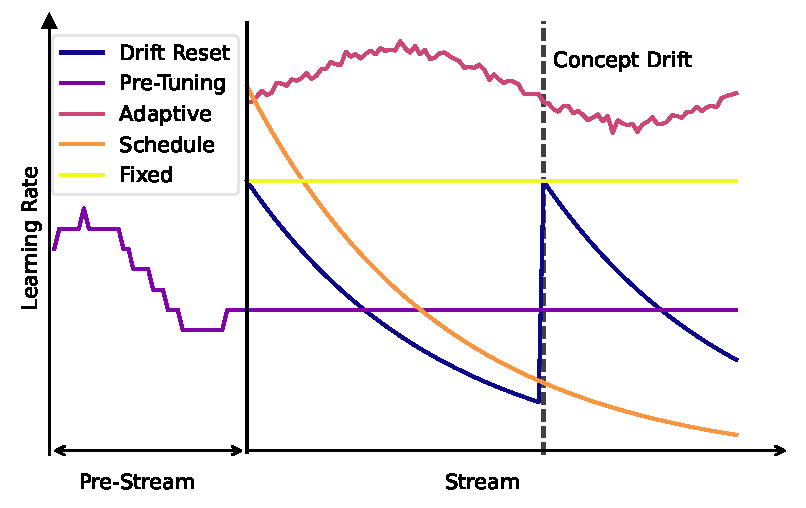
\includegraphics[width=0.9\textwidth]{figures/lr_overview.pdf}
   \caption{Overview of different learning rate optimization approaches.}
   \label{fig:lr_overview}
\end{figure}
In batch learning scenarios, where all training data is available a priori, the above methods are well researched.
Despite the increasing prevalence of online learning environments, where data becomes available as part of a data stream, their use in such scenarios has received little research attention.

According to \citet{bifetMOAMassiveOnline2010} a machine learning model operating on a data stream must be able to
\begin{enumerate}
   \item[R1:] process a single instance at a time,\label{rq:single_instance}
   \item[R2:] process each instance in a limited amount of time,\label{rq:limited_time}
   \item[R3:] use a limited amount of memory,\label{rq:limited_memory}
   \item[R4:] predict at any time,\label{rq:predict_any_time}
   \item[R5:] adapt to changes in the data distribution.\label{rq:adapt_to_drift}
\end{enumerate}

These requirements pose additional challenges in selecting an appropriate optimizer and learning rate.
To enable more informed decisions when optimizing the learning rate, we provide insight into these challenges and empirically evaluate commonly used optimization techniques in an online learning setting (i).
Furthermore, we introduce a \textit{drift reset} mechanism to adapt the learning rate to concept drifts that commonly occur in streaming environments (ii).
Finally, we propose a \textit{pre-tuning} approach to make effective use of any \textit{pre-stream} data that may be available prior to stream-based learning for the purpose of learning rate tuning (see Figure~\ref{fig:lr_overview}) (iii).

\section{Learning Rate in First-Order Optimization}

In the following, we will explain the theoretical background of the learning rate hyperparameter in first-order stochastic optimization.
First-order stochastic optimization algorithms, such as stochastic gradient descent, typically aim to solve the following problem
\begin{equation}
   \min_{\vtheta} \E_{\vx \sim \ptrain} [L(f(\vx; \vtheta), y)],
\end{equation}
where $L$ is a loss function that quantifies the prediction error of the model given model parameters $\vtheta$, data samples $\vx$ and their corresponding target outputs $y$, both sampled from the distribution $\ptrain$ defined by a set of training data.
The blueprint process for solving this problem using first-order stochastic optimization consists of the following steps for each iteration $t \in 0, \ldots, T$:
\begin{enumerate}
   \item Draw a mini-batch of samples $\vx_t$ from the distribution $p(\vx)$.
   \item Compute the loss $L_t = L(f(\vx_t; \vtheta_t), y_t)$ for examples $\vx_t$ with their respective labels $y_t$\footnotemark[1] and current parameters $\vtheta_t$.
   \item Compute gradient $\vg_t = \nabla_{\vtheta_t} L_t$ with respect to the parameters.
   \item Update the parameters for the next iteration using $\vg_t$ and possibly information from previous iterations.
\end{enumerate}

\footnotetext[1]{Note that for ease of notation we denote $\vx_t$ and $y_t$ as vectors and scalars even if they are typically mini-batches of multiple examples.}

For basic SGD, we can define the parameter update performed at the end of each iteration as
\begin{equation}\label{eq:sgd_update}
   \vtheta_{t+1}  = \vtheta_{t} - \eta_t \cdot \vg_t,
\end{equation}
where $\eta_t$ denotes the step size or \textit{learning rate} at timestep $t$.

The primary trade-off with respect to $\eta$ is that increasing it speeds up convergence, but also increases stochasticity and the risk of divergence~\citep{bengioPracticalRecommendationsGradientbased2012}.
In fact, \citet{smithBayesianPerspectiveGeneralization2018}, found that the “noise scale” of SGD is tied to $\eta$~\citep{smithBayesianPerspectiveGeneralization2018}.

\subsection{Learning Rate Schedules}

Often, the performance of a model can be improved by using a schedule that changes the learning rate as training progresses, yielding a vector of step sizes $\bm{\eta}$ that defines a step size $\eta_t$ for each timestep $t \in \{0, \ldots, T\}$~\citep{wuDemystifyingLearningRate2019b}.
For example, to ensure fast convergence early in training while mitigating jumping around potential minima later, it is common to use a decaying schedule that starts with a large learning rate and decreases over time.
An additional benefit of this approach is potentially better generalization, since larger learning rates can help skip sharp minima with poor generalization~\citep{hochreiterFlatMinima1997,chaudhariEntropySGDBiasingGradient2017}.

Commonly used forms of decay are exponential decay, where $\eta_{t}$ is calculated as
$\eta_{t} = \eta_1 \cdot \gamma^t$,
with $\gamma < 1$, and stepwise decay, which for a regular interval between steps of length $s$ is given as $\eta_1 \cdot \gamma^{\lfloor t/s \rfloor}$.
Another common approach is to decay $\eta$ each time the training loss plateaus for a given number of iterations. Other popular schedules include cyclic learning rates that oscillate $\eta$ between two values over a predefined interval.
For a triangular cycle, the learning rate is computed as
\begin{equation}
   \eta_t = \eta_1 + \frac{\hat{\eta} - \eta_1}{2s} \cdot \min_{i} \{|t-i\cdot s|\},
\end{equation}
where $\hat{\eta}$ is the learning rate at the midpoint of each cycle of length $s$.
Some studies~\citep{smithCyclicalLearningRates2017, smithSuperConvergenceVeryFast2018a} have found that cyclic schedules can significantly speed up the convergence of neural networks, in some cases even compared to adaptive techniques like Adam~\citep{kingmaAdamMethodStochastic2017b}.
While there are many alternatives, in this work we focus on exponential, step, and cyclic learning rates as some of the most commonly used generic schedules.
For a comprehensive overview and detailed analysis of learning rate policies, see \citet{wuDemystifyingLearningRate2019b}.

\subsection{Adaptive Learning Rates}

Several studies have proposed \textit{adaptive optimizers} that increase the robustness of the training process with respect to the learning rate.
These optimizers adjust the step size based on previous gradients at each optimization step~\citep{duchiAdaptiveSubgradientMethods2011}.

\begin{table}[ht]
   \centering
   \small
   \caption{
      Overview of additional time- and space-complexity of evaluated adaptive first-order optimizers compared to basic SGD.
      Values are given in big O notation with respect to the number of model parameters $D$.
   }\label{tab:param_free_optims}
   \begin{tabular}{@{}lllcc@{}}
      \toprule
      Optimizer                & Runtime            & Space             & Param. specific & LR free \\ \midrule
      AdaGrad                  & $\mathcal{O}(5D)$  & $\mathcal{O}(1D)$ & \cmark          & \xmark  \\
      Adam                     & $\mathcal{O}(12D)$ & $\mathcal{O}(2D)$ & \cmark          & \xmark  \\
      WNGrad                   & $\mathcal{O}(2D)$  & $\mathcal{O}(0)$  & \xmark          & \xmark  \\
      COCOB                    & $\mathcal{O}(14D)$ & $\mathcal{O}(4D)$ & \cmark          & \cmark  \\
      HD\footnotemark[2]       & $\mathcal{O}(2D)$  & $\mathcal{O}(1D)$ & \xmark          & \xmark  \\
      Mechanic\footnotemark[2] & $\mathcal{O}(10D)$ & $\mathcal{O}(1D)$ & \cmark          & \cmark  \\
      DoG                      & $\mathcal{O}(5D)$  & $\mathcal{O}(1D)$ & \xmark          & \cmark  \\
      D-Adapt\footnotemark[2]  & $\mathcal{O}(6D)$  & $\mathcal{O}(2D)$ & \xmark          & \cmark  \\
      \bottomrule
   \end{tabular}
\end{table}

One of the earlier techniques in this category is \textit{AdaGrad}~\citep{duchiAdaptiveSubgradientMethods2011}, which scales the learning rate based on the sum of squares of past gradients for each parameter, resulting in a parameter-specific step size.
Several other approaches, such as AdaDelta~\citep{zeilerADADELTAAdaptiveLearning2012a} and RMSProp, later built on AdaGrad's scaling approach.
The same is true for the widely used Adam optimizer~\citep{kingmaAdamMethodStochastic2017b}, which adds a momentum term from prior gradients to speed up convergence for parameters with consistent derivatives.
Another AdaGrad based optimizer is \textit{WNGrad}~\citep{wuWNGradLearnLearning2020}, which adaptively scales each parameter update based on the squared sum of past gradients.

\footnotetext[2]{Variant with SGD as the underlying optimizer.}

So-called \textit{parameter-free} gradient-based optimization approaches aim to eliminate the learning rate altogether by optimizing it as training progresses.
For example, the \textit{COCOB} algorithm~\citep{orabonaTrainingDeepNetworks2017} models parameter optimization as a gambling problem, where the goal is to maximize the reward from betting on each gradient.
The resulting strategy is equivalent to running a meta-optimization algorithm that estimates the expected optimal learning rate~\citep{orabonaTrainingDeepNetworks2017}.
Several other studies~\citep{vanervenMetaGradMultipleLearning2016a,baydinOnlineLearningRate2018,cutkoskyMechanicLearningRate2023} have also used the idea of learning $\eta$ via a meta-optimization process.
The \textit{hypergradient descent} (HD) approach~\citep{baydinOnlineLearningRate2018}, for example, adapts the learning rate of a base optimizer like SGD using a meta-gradient descent procedure, although this does not remove the learning rate entirely, but replaces it with a less sensitive hypergradient step size.
Mechanic~\citep{cutkoskyMechanicLearningRate2023} pursues the same goal by applying a meta \textit{online convex optimization} (OCO) algorithm to an arbitrary base optimizer.

Research has shown that in an OCO problem setting with stationary data, the worst-case optimal fixed step size for SGD is
\begin{equation}\label{eq:oco_optimal_lr}
   \eta^* = \frac{||\vtheta_1 - \vtheta^*||}{\sqrt{\sum_{t=1}^{n} ||\vg_t||^2}}.
\end{equation}
Multiple parameter-free optimizers, make use of this notion.
As its name suggests, the \textit{Distance over Gradients} (DoG)~\citep{ivgiDoGSGDBest2023} algorithm estimates the unknown numerator in \Eqref{eq:oco_optimal_lr} as the maximum distance $\max_{i<t}||\vtheta_1 - \vtheta_i||$ between the initial parameters and the parameters of all previous iterations.
DoG additionally uses polynomial decay averaging as proposed by~\citet{shamirStochasticGradientDescent2012}.
\textit{D-Adaptation} by \citet{defazioLearningRateFreeLearningDAdaptation2023a}, on the other hand, employs weighted dual averaging~\citep{duchiDualAveragingDistributed2012} to compute bounds on the distance between initial and optimal parameters.
Although adaptive optimization techniques seem intuitively well suited for non-stationary data, their application to data streams has rarely been investigated.
Therefore, we assess the suitability of some of the most prominent adaptive optimizers, listed in Table~\ref{tab:param_free_optims}, for stream-based learning.

\section{Learning Rate in Online Learning}

In a batch learning setting, optimizing the learning rate involves minimizing the expected loss on a hold-out set of validation data.
Formally, we can express this task as
\begin{equation}
   \label{eq:batch_lr_optim}
   \min_{\bm{\eta}} \E_{(\vx, y) \sim \hat{p}_{\rm{val}}} L(f(\vx; \vtheta_n), y),
\end{equation}
where samples $(\vx, y)$ are drawn from a distribution $\hat{p}_{\rm{val}}$ defined by a validation dataset and $\vtheta_n$ are the model parameters at the end of training that depend on the learning rate schedule $\bm{\eta}$.
In online learning where data is generated incrementally, this notion of learning rate optimization is not feasible.
Due to requirements \textbf{R1-R5}, models operating in an online learning environment should be evaluated in a \textit{prequential} manner~\citep{bifetMOAMassiveOnline2010}, where each sample $\vx_t$ in the data stream is first used to test and then to train the model, ensuring that testing is done on previously unobserved data.

Training in such a scenario can be more accurately modeled as an online convex optimization problem~\citep{shalev-shwartzOnlineLearningOnline2011,hazanIntroductionOnlineConvex2016}, where the optimizer suffers a loss $L(f(\vx; \vtheta_t), y)$ and produces updated parameters $\vtheta_{t+1}$ at each iteration of the data stream.
Learning rate optimization in this setting can be formulated as
\begin{equation}
   \label{eq:stream_lr_optim}
   \min_{\bm{\eta}} \sum_{t=1}^{n} \E_{(\vx, y) \sim \hat{p}_{\rm{stream}}^{(t)}} L(f(\vx; \vtheta_t), y).
\end{equation}

Compared to \Eqref{eq:batch_lr_optim}, \Eqref{eq:stream_lr_optim} features some key differences.
Due to the requirement to be able to predict at any time (\textbf{R4}), the goal is to minimize the expected total sum of losses over all timesteps of the prequential evaluation process, instead of the validation loss for the final parameters $\vtheta_n$.
Therefore, the speed of convergence is more important in the streaming setting, while the performance of the final $\vtheta_n$ parameter has a much smaller impact.
Since memory is limited (Requirement~\ref{rq:limited_memory}), it is also not possible to continue training on previously observed data as long as the loss decreases, which puts even more emphasis on fast adaptation.
At the same time, a higher learning rate that temporarily increases the loss by skipping local minima may be suboptimal with respect to \Eqref{eq:stream_lr_optim}, even if it eventually leads to a lower loss.
Another difference to conventional batch learning is that the data distribution $\hat{p}_{\rm{stream}}^{(t)}$ is time-dependent, due to the fact that streams are often subject to distributional changes such as \textit{concept drifts} over time \citep{widmerLearningPresenceConcept1996}.
While other forms of drifts exist, we use \textit{concept drift} as an umbrella term for any kind of distributional shift in the following.

\subsection{Learning Rate Tuning}\label{subsec:pre-tuning}

Although strict online learning assumes that no data is available prior to the deployment of a model in the streaming environment, smaller amounts of data may be available prior to the stream learning process in practical scenarios.
Such data can then be used to tune the learning rate of the model before stream deployment.
However, the differences in evaluation schemes described above may cause conventional learning rate tuning to produce poor results for stream-based learning.
In offline learning, learning rate tuning is typically performed by repeating the training process for a grid of possible parameter values and selecting the value that yields the best target metric on a held-out validation set after the training is completed.
As a result of only considering the performance at the end and not throughout the training process, this tuning approach may result in poor results with respect to the goal of learning rate optimization in streaming environments (see \Eqref{eq:stream_lr_optim}).
Therefore, we propose the modified tuning approach described in \Cref{alg:pre-tuning} aimed at approximating \Eqref{eq:stream_lr_optim}, which we call learning rate \textit{pre-tuning}.

\begin{algorithm}
   \caption{Learning Rate Pre-Tuning}\label{alg:pre-tuning}
   \begin{algorithmic}[1]
      \Require Set of learning rate values $\sH$, set of schedule parameter values $\sG$, data samples $\sX$
      \Require Optimization function $o$, metric function to tune $m$, number of tuning steps $n_{\rm{steps}}$

      \State $\sS \gets \{(\vx_i, y_i) \sim \hat{p}_{\sX}| \forall i \in \{1, \ldots, n_{\text{steps}}\} \}$ \Comment{Create artificial stream by sampling $\sX$ with replacement.}
      \State $v^* \gets -\infty$
      \For{$\eta$ \textbf{in} $\sH$, $\gamma$ \textbf{in} $\sG$}
      \State $v \gets v_{\textrm{init}}$ \Comment{Initialize metric value.}
      \For{$\vx, y$ \textbf{in} $\sS$}
      \State $\hat{y} \gets f(\vx, \vtheta)$ \Comment{Calculate predictions with model function $f$.}
      \State $v \gets m(\hat{y}, y, v)$ \Comment{Update metric value.}
      \State $\vg \gets \nabla_{\vtheta} L(\hat{y}, y)$ \Comment{Calculate gradient of predictive loss w.r.t. $\vtheta$.}
      \State $\vtheta, \eta \gets o(\vtheta, \vg, \eta, \gamma)$ \Comment{Update model parameters $\vtheta$ and learning rate $\eta$.}
      \EndFor
      \If{$v > v^*$}
      \State $\eta^* \gets \eta$ \Comment{Update best learning rate.}
      \State $\gamma^* \gets \gamma$ \Comment{Update best schedule parameters.}
      \EndIf
      \EndFor
      \State \textbf{return} $\eta^*, \gamma^*$ \Comment{Return best hyperparameter values.}
   \end{algorithmic}
\end{algorithm}

To emulate the data stream to be processed after tuning, we continuously draw samples with replacement from the tuning data $\sX$ in a bootstrapping procedure instead of training on all data for multiple epochs.
By doing so, we aim to increase the variability of the data and thus the similarity to a real data stream.
We then optimize the learning rate and any optional learning rate schedule parameters $\gamma$ with respect to the selected performance metric $m$ over the emulated stream $\sS$.
While we use a simple grid search for this purpose in \cref{alg:pre-tuning}, any parameter search technique could be used here.
We provide a detailed experimental evaluation of our approach in Section~\ref{sec:experiments}.


\subsection{Concept Drift Adaptation}

Concept drift requires repeated adaptation of the model parameters.
If post-drift training is interpreted as a new online optimization problem, the worst-case optimal learning rate can be computed according to \Eqref{eq:oco_optimal_lr}, replacing the initial parameter values $\vtheta_1$ with the values at the time of drift onset $\vtheta_{t_{\rm{drift}}}$.
As a result, stronger drifts that cause $\vtheta^*$ to move away from $\vtheta_{t_{\rm{drift}}}$ can benefit from larger learning rates.

Based on this notion, we propose a simple adaptation to decaying learning rate schedules that resets $\eta$ to its original value when a concept drift is detected.
An exponential schedule modified with our approach will thus yield learning rates of
\begin{equation}
   \eta_t = \eta_1 \cdot \gamma^{t-t_{\rm{drift}}},
\end{equation}\label{eq:drift_reset}
where $t_{\rm{drift}}$ marks the timestep at which the drift was last detected.
For drift detection, we apply either ADWIN~\citep{bifetLearningTimeChangingData2007} or the Kolmogorov-Smirnov test~\citep{masseyKolmogorovSmirnovTestGoodness1951} to the prequential losses.
To avoid mistakenly detecting loss decreases as concept drift, we test only for increases of the prequential loss.

Our approach is similar to some \textit{forgetting mechanisms} commonly used in conventional online learning~\citep{gamaSurveyConceptDrift2014}.
To improve model plasticity, such mechanisms partially or completely reset the current model parameters to their initial values.
However, we hypothesize that this approach is not well suited for neural-based approaches.
The reason is that, under the assumption of convexity, the newly initiated parameters must be closer to the optimal parameters $\vtheta^*$ than the current parameters to be beneficial.
We experimentally compare our approach with this weight-reset mechanism in Section~\ref{sec:experiments}.

\section{Experiments}\label{sec:experiments}

We empirically evaluate our hypotheses using the following setup\footnote[3]{Code available at \url{anonymous.4open.science/r/LODL-D458/}.}:

We use both synthetic and publicly available real-world classification datasets with different sizes and types of concept drift, listed in Table~\ref{tab:datasets}.
Our evaluations include two synthetic \textit{Random Radial Basis Function} (RBF) datasets that we manipulated to incorporate concept drift using the online learning framework \textit{River}~\citep{montielRiverMachineLearning2020a}.

\begin{table}[ht]
   \centering
   \small
   \caption{Datasets used for experimental evaluations.}
   \begin{tabular}{@{}clcccc@{}}
      \toprule
      Type                    & Data Stream              & Instances               & Features & Classes \\
      \midrule
      \multirow{4}{*}{Synth.} & Agrawal                  & 100,000                 & 9        & 2       \\
                              & LED                      & 100,000                 & 7        & 10      \\
                              & RBF\textsubscript{a}     & 100,000                 & 20       & 5       \\
                              & RBF\textsubscript{i}     & 100,000                 & 20       & 5       \\
      \midrule
      \multirow{5}{*}{Real}   & Covertype                & 100,000\footnotemark[4] & 54       & 7       \\
                              & Electricity              & 45,312                  & 8        & 2       \\
                              & Insects\textsubscript{a} & 52,848                  & 33       & 6       \\
                              & Insects\textsubscript{g} & 24,150                  & 33       & 6       \\
                              & Insects\textsubscript{i} & 57,018                  & 33       & 6       \\
      \bottomrule
   \end{tabular}
   \label{tab:datasets}
\end{table}

\footnotetext[4]{For Covertype we use only the first 100,000 from a total of 581,012 instances.}

We further employ the \textit{Electricity} and \textit{Covertype}~\citep{misc_covertype_31} datasets, which are commonly used to evaluate online learning models, as well as two \textit{Insects} datasets~\citep{souzaChallengesBenchmarkingStream2020} with predefined types of concept drift.
\textit{Covertype} is available on \textit{OpenML}~\citep{vanschorenOpenMLNetworkedScience2014}, while the remaining datasets are part of River.
We limit our investigations to multi-layer perceptrons (MLPs) with a single-hidden-layer and hidden units matching the number of input features implemented with \textit{PyTorch}~\citep{paszkePyTorchImperativeStyle2019}.
Even though more elaborate architectures could in theory produce better results, they also typically require more tuning and longer training than smaller models making them less suited for streaming environments from a practical standpoint.

We tune the base learning rate $\eta_1$ of all but the parameter-free approaches using a grid search of ten geometrically spaced values and configure adaptive optimizers with their default parameter values. For HD, Mechanic and D-Adaptation we select SGD as the base algorithm.
We select a fixed factor $\gamma$ for decay schedules on all datasets.
For the proposed learning rate resetting mechanism, we select a smaller decay factor and set the confidence level $\delta$ for drift detection to $10^{-4}$.
For our evaluations we process each dataset sequentially, emulating streams of mini-batches of four instances each, while recording the prequential accuracy and other metrics in intervals of 25 iterations.
We report our results averaged over five random seeds.

\subsection{Learning Rate Schedules}

To evaluate the effectiveness of our learning rate resetting mechanism for drift adaptation (see \Eqref{eq:drift_reset}), we compare its average prequential accuracy to that of model weight resetting, commonly used in online learning.

\begin{table}[ht]
   \centering
   \small
   \caption{Average prequential accuracy [\%] for static and drift adaptive learning rate schedules with SGD. LR-Reset\textsubscript{A} uses ADWIN, LR-Reset\textsubscript{K} Kolmogorov-Smirnov testing for drift detection. Best values are shown in \textbf{bold}, values within the $1\sigma$ interval of best values \underline{underlined}.}
   \begin{tabular}{llllllllll}
      \toprule
      Schedule        & Agrawal               & LED                 & RBF\textsubscript{a}   & RBF\textsubscript{i} & Covertype             & Electricity           & Insects\textsubscript{a} & Insects\textsubscript{g} & Insects\textsubscript{i} \\
      \midrule

      Fixed           & \bfseries 79.78±1.09  & \bfseries 73.91±.04 & \bfseries 89.57±2.61   & 57.18±2.69           & \underline{83.42±.50} & \bfseries 73.77±.40   & 71.50±.08                & 75.31±.21                & 60.48±.20                \\
      Exp.            & 77.98±1.36            & 73.38±.14           & \underline{87.66±3.53} & 50.75±1.38           & 82.95±.26             & \underline{73.51±.48} & \underline{72.19±.37}    & \bfseries 75.91±.14      & \bfseries 61.28±.16      \\
      Step            & 76.56±1.13            & 72.86±.18           & 84.98±6.46             & 50.69±1.93           & 82.89±.37             & \underline{73.62±.53} & \bfseries 72.23±.27      & \underline{75.83±.21}    & \underline{61.18±.11}    \\
      Cyclic          & \underline{78.72±.90} & 73.67±.17           & \underline{88.40±4.26} & 58.67±1.63           & \bfseries 83.44±.08   & 68.38±.81             & 71.74±.39                & 75.64±.06                & 60.48±.20                \\
      Weight-Reset    & 72.03±.91             & 64.31±2.16          & 70.41±.92              & \bfseries 61.07±.76  & 82.92±.57             & 71.17±.62             & 63.55±.42                & 69.66±.65                & 49.97±.67                \\
      LR-Reset (Ours) & 78.26±.73             & 72.95±.13           & \underline{87.60±3.43} & 52.88±1.72           & 82.92±.32             & 73.07±.66             & 71.48±.34                & 75.54±.11                & 60.39±.18                \\
      %TODO: Add LR-Reset with KSWIN drift detection
      \bottomrule
   \end{tabular}
   \label{tab:lr_resetting}
\end{table}

As can be seen in Table~\ref{tab:lr_resetting}, our approach clearly outperforms weight-resetting on all but \textit{Covertype}, but rarely yields an advantage over a static schedule.
Since both variants our resetting approach perform similarly, this performance gap is likely not caused by the drift detector.
Rather, it appears that using a larger initial learning rate and slower decay is sufficient to ensure adequate adaptability to concept drift throughout a data stream, while providing better stability in later stages.
Overall, a slower but static decay paired with a larger initial learning rate seems to be preferable to a more aggressive schedule with our drift resetting mechanism, unless severe concept drift as in \textit{RBF incremental} is expected.

With accuracy values within $1\sigma$ of each other on all evaluated streams, the stepwise decay shows almost identical performance to the exponential decay.
The accuracy of the cyclic schedule for \textit{RBF incremental} and \textit{Covertype}, on the other hand, significantly outperforms the other static and adaptive schedules, but lags behind on all other streams.
We also did not find an order of magnitude improvement in convergence speed as observed by~\citep{smithSuperConvergenceVeryFast2018a} for the scenario studied.

\def\asize{0.5\textwidth}
\begin{figure}[ht]
   \centering
   \begin{subfigure}[b]{\asize}
      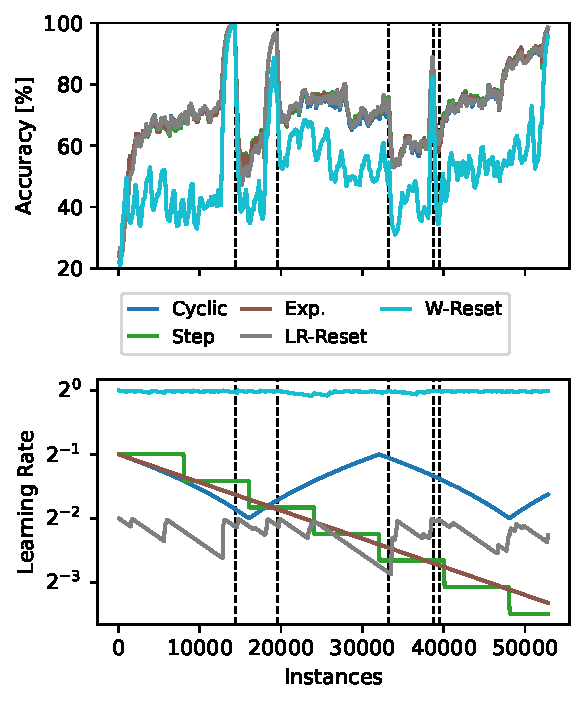
\includegraphics[width=\textwidth]{figures/lr_norms_schedules_insects_abrupt.pdf}
      \caption{Schedules}
      \label{fig:prequential_schedulers_insects}
   \end{subfigure}
   \begin{subfigure}[b]{0.99\textwidth - \asize}
      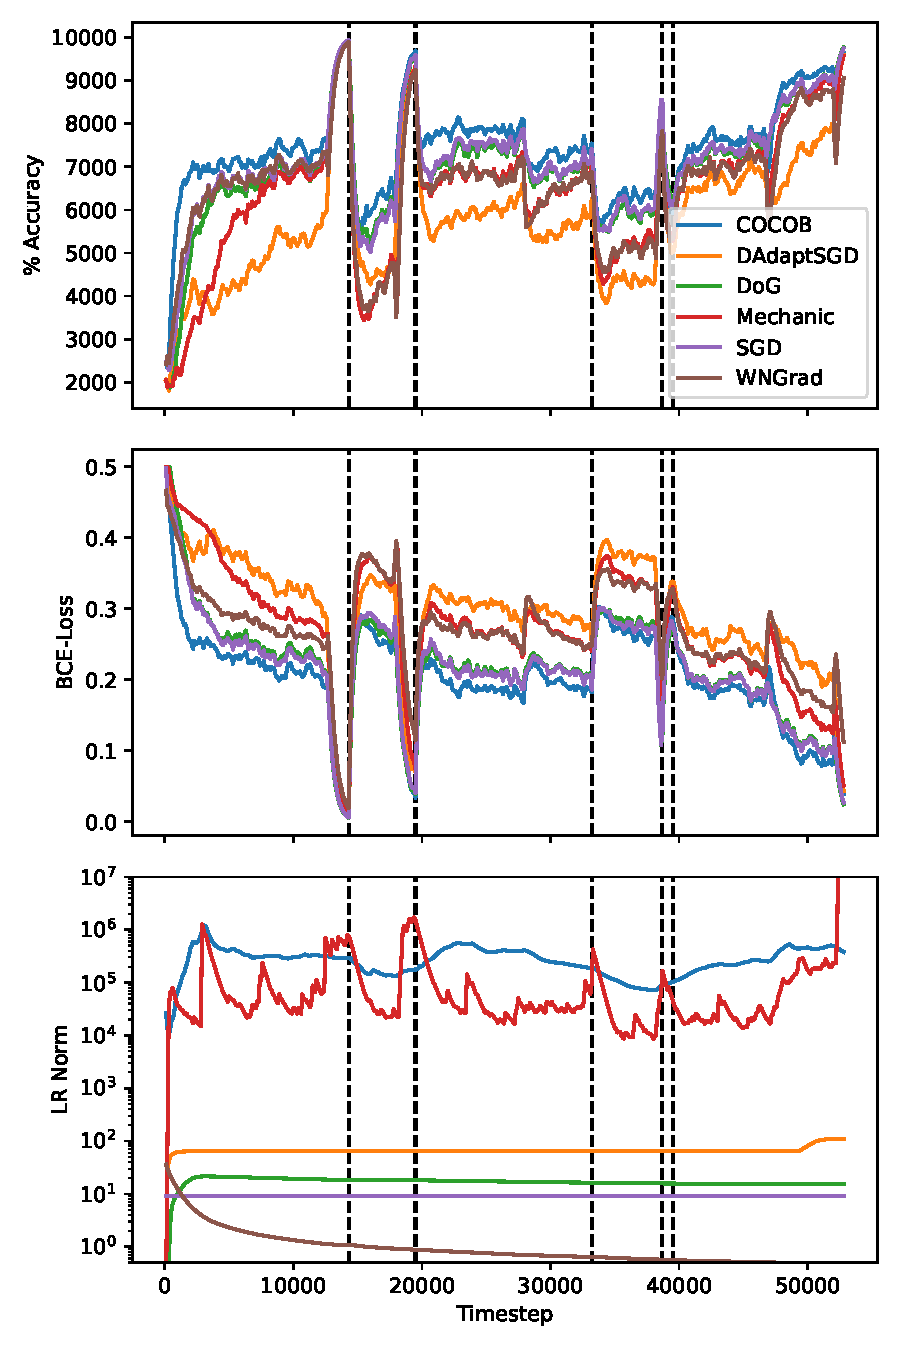
\includegraphics[width=\textwidth]{figures/lr_norms_optims_insects_abrupt.pdf}
      \caption{Adaptive Optimizers}
      \label{fig:prequential_optims_insects}
   \end{subfigure}
   \caption{Prequential accuracy and learning rate for different schedules and adaptive optimizers on \textit{Insects\textsubscript{a}} dataset. Concept drifts are marked by dashed lines. Accuracy is exponentially smoothed with a decay factor of 0.75.}
\end{figure}

\subsection{Adaptive Learning Rates}

Our results for adaptive optimizers displayed in Table~\ref{tab:results_adaptive_optims}, show a strong data dependency as none of the evaluated algorithms significantly outperforms its competitors on average.
However, since SGD yields the best accuracy on \textit{RBF\textsubscript{a}} but is clearly surpassed on \textit{Insects\textsubscript{a}}, the type of concept drift does not seem to be significant.
Due to its simplicity and favorable computational efficiency, it appears that SGD should be selected out of the non-parameter-free approaches in most cases.
The SGD variant of Hypergradient Descent (HD)~\citep{baydinOnlineLearningRate2018} and WNGrad~\citep{wuWNGradLearnLearning2020} on the other hand seem to rarely be optimal choices.

\begin{table}[ht]
   \centering
   \small
   \caption{Average prequential accuracy [\%] for different optimizers. Best values are shown in \textbf{bold}, values within the $1\sigma$ interval of best values \underline{underlined}.}
   \begin{tabular}{lllllllllll}
      \toprule
                                                         & Optimizer & Agrawal              & LED                 & RBF\textsubscript{a} & RBF\textsubscript{i} & Covertype           & Electricity         & Insects\textsubscript{a} & Insects\textsubscript{g} & Insects\textsubscript{i} \\
      \midrule
      \multirow{5}{*}{\rotatebox[origin=c]{90}{Tuned}}   & SGD       & \bfseries 79.64±2.03 & \bfseries 73.91±.04 & \bfseries 89.57±2.61 & \bfseries 57.18±2.69 & \bfseries 83.42±.50 & 73.77±.40           & 71.50±.08                & 75.31±.21                & 60.48±.20                \\
                                                         & Adam      & \bfseries 78.91±2.40 & \bfseries 73.98±.20 & 86.33±1.85           & \bfseries 60.32±3.75 & 79.01±.27           & 69.79±.54           & \bfseries 75.38±.24      & 75.78±.74                & \bfseries 64.17±.13      \\
                                                         & AdaGrad   & \bfseries 79.13±1.62 & 72.55±.31           & 81.92±3.89           & 45.00±1.55           & 81.68±.35           & 76.99±1.20          & 74.87±.40                & 77.15±.27                & 62.51±.59                \\
                                                         & WNGrad    & 76.91±.47            & 64.66±.34           & 80.07±.67            & 42.06±.43            & 76.98±.15           & 70.80±.59           & 66.25±.19                & 66.75±.40                & 56.14±.21                \\
                                                         & HD        & \bfseries 80.19±1.56 & 73.81±.09           & \bfseries 89.78±3.37 & 56.37±5.01           & \bfseries 83.36±.25 & 73.83±.32           & 70.67±.06                & 73.37±.21                & 59.92±.18                \\ \midrule
      \multirow{4}{*}{\rotatebox[origin=c]{90}{LR-Free}} & COCOB     & 78.21±1.12           & \bfseries 73.88±.50 & \bfseries 90.75±1.28 & 51.70±2.11           & 82.27±.46           & \bfseries 84.48±.88 & 74.75±.11                & \bfseries 77.67±.17      & 63.93±.17                \\
                                                         & DoG       & \bfseries 78.77±2.25 & 73.34±.13           & 87.04±3.13           & 55.72±2.43           & 83.07±.64           & 71.53±.70           & 70.59±.26                & 74.01±.21                & 59.66±.22                \\
                                                         & DAdapt    & 60.16±.96            & 54.69±8.34          & 41.37±3.34           & 42.61±1.46           & 76.69±.79           & 66.03±1.75          & 50.05±11.26              & 48.21±10.62              & 36.00±11.81              \\
                                                         & Mechanic  & 62.09±9.20           & 69.04±.19           & 87.33±.50            & 44.45±.85            & 78.67±.18           & 50.73±7.60          & 55.31±21.47              & 65.80±.53                & 47.89±17.46              \\
      \bottomrule
   \end{tabular}
   \label{tab:results_adaptive_optims}
\end{table}
In the category of learning rate free optimizers COCOB~\citep{orabonaTrainingDeepNetworks2017}, outperformed its competitors on all but two datasets.
It comes close to or even exceeds the best tuned approaches in terms of accuracy.
Although yielding lower accuracy on average, DoG also comes within reach of the tuned methods, while offering much better runtime and memory efficiency compared to COCOB (see Table~\ref{tab:param_free_optims}).
Mechanic~\citep{cutkoskyMechanicLearningRate2023} and D-Adaptation~\citep{defazioLearningRateFreeLearningDAdaptation2023a} performed significantly worse than their competitors on the evaluated streams.

The learning rate curves shown in Figure~\ref{fig:prequential_schedulers_insects}, provide an indication regarding the reason for the poor performance of WNGrad and D-Adaption.
Whereas the learning rate of DoG quickly approaches the optimal learning rate, WNGrad and D-Adaptation diverge considerably from it.

The learning rate of the best performing Adam exhibits spikes for most change points, suggesting some form of adaptability to drift.
However, since the much worse performing Mechanic shows similar spikes, this is unlikely to be contributing significantly to Adam's high accuracy on \textit{Insects\textsubscript{a}}.
Instead, it likely stems from its second moment scaling, which is also a feature of the similarly performing AdaGrad.

It may also be noted that the learning rates of the COCOB, Adam and Mechanic optimizers with parameter-specific learning rates exceed those of single value step sizes by multiple orders of magnitude.
This is an effect of second moment scaling, which creates larger learning rates for parameters with small and consistent gradients~\citep{cutkoskyMechanicLearningRate2023}.
Therefore, the norms of parameter updates generated by these approaches are not necessarily larger.


\subsection{Learning Rate Tuning}

We evaluate our pre-tuning approach by using either 500 or 1000 instances held out at the beginning of each stream for tuning. We assess Multi-Layer Perceptrons (MLPs) with 64 or 128 hidden units per layer and either one or three hidden layers.
Although our technique consistently performed well across all architectures, we specifically highlight the smallest network as it best represents resource-critical streaming applications. For an overview of results across all architectures, please refer to our supplementary material.

To determine the learning rate and decay factor, we rely on the optimal mean prequential accuracy. This choice accounts for the potential bias towards learning rates associated with lower initial losses, as loss values often decrease notably during training.

\begin{figure}[hb]
   \centering
   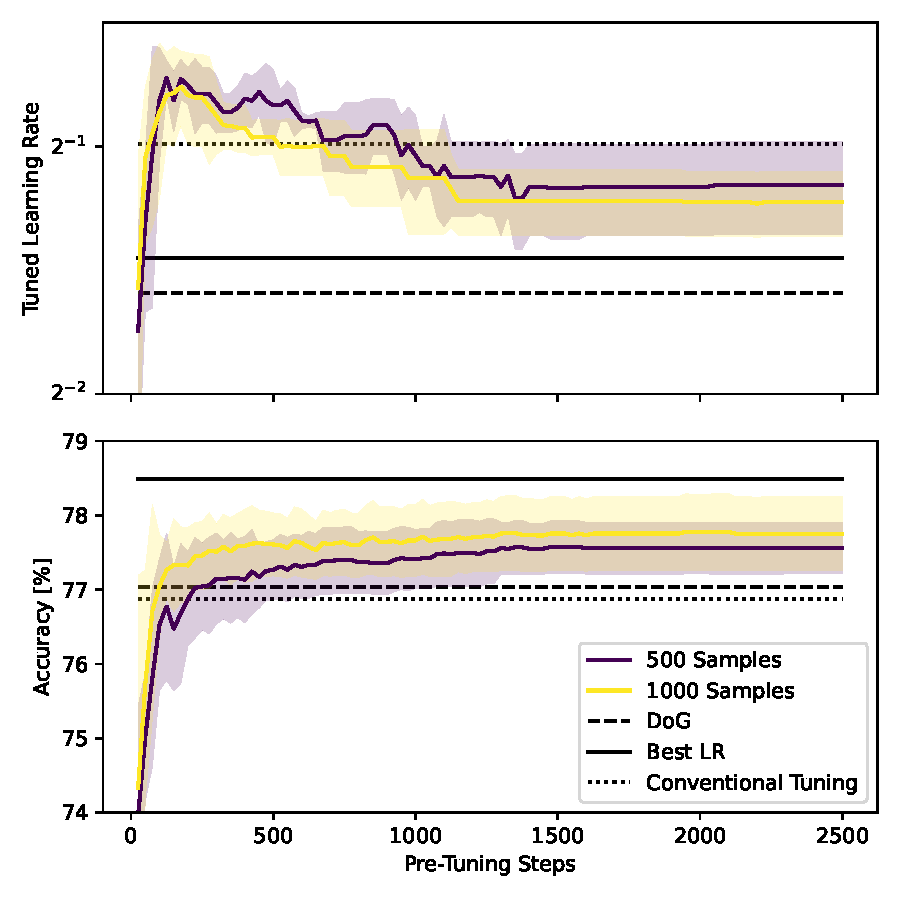
\includegraphics[width=\textwidth]{figures/pretune_1x64_acc_lr_exp_schedule.pdf}
   \caption{Absolute difference between pre-tuned and optimal learning rate and resulting accuracy on data streams for SGD and an exponential learning rate schedule with 500 or 1000 tuning samples. DoG is not included in first subplot since it is not intended for use with LR decay. Results are averaged over all real-world datasets. The shaded area represents the 1$\sigma$-interval.}\label{fig:pretune_lr_accuracy}
\end{figure}
Figure~\ref{fig:pretune_lr_accuracy} shows the absolute difference between the learning rate resulting from the pre-tuning process and the optimal value $|\eta_p - \eta^*|$ at each tuning step averaged over all real-world datasets.
Batch tuning with 800 training and 200 validation samples initially yields a better approximation of the optimal learning rate. However, our streaming-specific approach undercuts the baseline after 1000 tuning steps, consistently decreasing and ultimately reaching approximately half of the approximation error observed in batch tuning.
The performance also remains nearly identical, even when using only 500 samples for tuning, which demonstrates the data efficiency of pre-tuning.
The superior performance of our approach is also reflected in the accuracy scores depicted in the right subfigure of Figure~\ref{fig:pretune_lr_accuracy}.
In fewer than 1000 steps, our approach comes closer to the optimal learning rate and also exceeds the accuracy of conventional tuning.
Notably, our approaches usage of the average prequential accuracy more accurately resembles the online learning process and sets it apart from conventional tuning, which solely focuses on performance at the end of the tuning process.
Pre-Tuning also surpasses DoG, which we selected as a baseline due to being the best performing parameter-free technique within the group of optimizers with a global learning rate that are the most comparable to our approach.
This advantage comes despite a smaller average absolute deviation of DoG compared to our approach, which can be explained by the fact that DoG strongly underestimates the optimal learning rate at the beginning of training (see e.g. \Cref{sub@fig:prequential_optims_insects}), where fast adaptation is crucial.
Because DoG closely approaches the best learning rate for the majority of the stream, this effect is barely reflected in the average deviation.

\begin{table}[ht]
   \centering
   \small
   \caption{
      Mean prequential accuracy of learning rate tuning approaches.
   }\label{tab:lr_tuning}
   \begin{tabular}{llllllllll}
      \toprule
      Approach                       & Agrawal             & LED                 & RBF\textsubscript{a} & RBF\textsubscript{i} & Covertype             & Electricity           & Insects\textsubscript{a} & Insects\textsubscript{g} & Insects\textsubscript{i} \\
      \midrule
      Oracle                         & 83.70               & 73.95               & 93.84                & 81.52                & 83.14                 & 74.15                 & 71.98                    & 75.28                    & 60.75                    \\
      COCOB                          & 83.71±.25           & 74.34±.09           & 95.29±.24            & 78.59±.38            & 82.96±.19             & 84.57±.08             & 75.39±.10                & 77.62±.08                & 64.02±.11                \\ \midrule
      DoG                            & 82.06±.52           & \bfseries 73.71±.11 & 91.36±.46            & \bfseries 77.63±1.24 & \bfseries 82.56±.15   & 70.47±.40             & 70.59±.10                & 73.92±.11                & 58.83±.07                \\
      Batch Tuning                   & 81.09±1.34          & 66.67±3.28          & 91.89±.39            & 72.51±1.63           & \underline{82.41±.61} & 72.86±.76             & 69.81±2.18               & 73.91±.64                & 58.27±2.21               \\
      Pre-Tuning\textsubscript{500}  & 82.01±.32           & 73.26±.03           & \bfseries 92.36±.03  & 72.98±.44            & 80.25±1.86            & \underline{73.34±.45} & \bfseries 71.81±.04      & \bfseries 75.22±.08      & \bfseries 60.55±.10      \\
      Pre-Tuning\textsubscript{1000} & \bfseries 82.56±.25 & 73.30±.00           & 92.18±.38            & 73.19±.31            & 80.80±1.05            & \bfseries 73.37±.34   & \bfseries 71.81±.06      & \underline{75.17±.05}    & 60.33±.28                \\
      \bottomrule
   \end{tabular}
\end{table}


In conclusion, our proposed tuning approach enables significantly better learning rate selection for prequential evaluation on data streams compared to both conventional tuning and DoG.
Additionally, pre-tuning has the benefit that once completed, no additional memory or runtime costs are incurred.
In streaming applications, where computing resources are often times a limiting factor, this could be a critical advantage.
However, if computational efficiency is insignificant, the highly performant but expensive COCOB~\citep{orabonaTrainingDeepNetworks2017} or the slightly less performant and much less expensive DoG~\citep{ivgiDoGSGDBest2023} may be more appropriate.
The usefulness of our pre-tuning approach is also likely to be limited in cases where the available tuning data is not representative for the subsequent data stream, which would for example be the case for data streams with extreme concept drift.
In such cases, approaches with a dynamic learning rate are presumably superior.

\section{Conclusion}

In this work, we investigate the influence and selection of the learning rate and optimization procedure with respect to training neural networks in streaming environments.
We first provide theoretical background on discrepancies between learning rate optimization in conventional batch learning and online learning.
Based on these differences, we derive a simple mechanism resetting the learning rate on concept drift occurrences.
We then give an overview learning rate free algorithms popular in batch learning, which we compare experimentally on multiple synthetic and real-world datasets,
finding both COCOB and DoG to come close to the performance of optimizers with tuned learning rates.
Lastly, we introduce a streaming specific learning rate tuning approach that grants significant performance increases over conventional tuning via a train-validation split.

\bibliography{collas2024_conference}
\bibliographystyle{collas2024_conference}

\appendix
\section{Appendix}
You may include other additional sections here.

\end{document}
